% Created 2021-04-22 Thu 17:52
% Intended LaTeX compiler: pdflatex
\documentclass[twocolumn]{article}
\usepackage[utf8]{inputenc}
\usepackage[T1]{fontenc}
\usepackage{graphicx}
\usepackage{grffile}
\usepackage{longtable}
\usepackage{wrapfig}
\usepackage{rotating}
\usepackage[normalem]{ulem}
\usepackage{amsmath}
\usepackage{textcomp}
\usepackage{amssymb}
\usepackage{capt-of}
\usepackage{hyperref}
\usepackage[margin=0.5in]{geometry}
\author{Hee Hwang and Sudarshan Raghavan}
\date{\today}
\title{Data Augmentation for Improved Generalizability of Natural Language Processing Models}
\hypersetup{
 pdfauthor={Hee Hwang and Sudarshan Raghavan},
 pdftitle={Data Augmentation for Improved Generalizability of Natural Language Processing Models},
 pdfkeywords={},
 pdfsubject={},
 pdfcreator={Emacs 26.3 (Org mode 9.1.9)}, 
 pdflang={English}}
\begin{document}

\maketitle
\begin{abstract}
A rapid data augmentation framework to improve the performance of natural language processing models. To augment data for a particular downstream task, we use DepCC, A Dependency-Parsed Text Corpus from Common Crawl. First, we take the Common Crawl data and index 35M documents using Apache Solr, a search engine that uses BM25(Similar to TF-IDF) scoring model. Secondly, we prepare queries from the train/test dataset. After retrieving relevant documents using the query, we convert the documents into dense embeddings and apply  K-nearest-neighbors to the candidate passages to rank the relevant documents. We augment data using various strategies. To show performance, we measure held-out accuracy.
\end{abstract}

\section{Datasets}
\label{sec:org8461f64}
\begin{itemize}
\item ACL  : Citation Intent Classification
\item Hyper: HyperPartisan News Detection
\item IMDb : Sentiment Classification
\end{itemize}
\subsection{Size of Datasets}
\label{sec:org295db5f}
\begin{center}
\begin{tabular}{lrrrr}
\hline
Task & train set & dev set & test set & \# of Classes\\
\hline
ACL & 1688 & 114 & 139 & 6\\
\hline
Hyper & 516 & 64 & 65 & 2\\
\hline
IMDb & 20000 & 5000 & 25000 & 2\\
\hline
\end{tabular}
\end{center}

\subsection{Size of Augmented data}
\label{sec:org484f24b}
\begin{center}
\begin{tabular}{lrrrr}
\hline
Task & Baseline & Strat. (i) & Strat. (ii) & Strat. (iii)\\
\hline
ACL & 1688 & 11005 & 10248 & 10621\\
\hline
Hyper & 516 & 1496 & 2184 & 2184\\
\hline
IMDb & 20000 & 29492 & 67004 & 68666\\
\hline
\end{tabular}
\end{center}


\section{Results}
\label{sec:org14ae7f1}
\begin{center}
\begin{tabular}{lrrrr}
\hline
Task & Baseline & Strat. (i) & Strat. (ii) & Strat. (iii)\\
\hline
ACL & 62.5 & 60.5 & 64.4 & 67.1\\
\hline
Hyper & 85.2 & 90.2 & 88.7 & 86.7\\
\hline
IMDb & 93.8 & 92.4 & 91.9 & 92.3\\
\hline
\end{tabular}
\end{center}

\section{Baseline models:}
\label{sec:org103a0d1}
\begin{itemize}
\item An off-the-shelf RoBERTa model that has been finetuned to perform classification for each of the downstream tasks
\end{itemize}

\section{Augmentation Model}
\label{sec:org919a13a}
\begin{center}
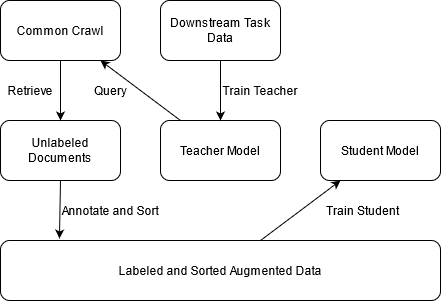
\includegraphics[width=.9\linewidth]{./png/da.png}
\end{center}

\section{Algorithm}
\label{sec:orgde2d53c}
\begin{verbatim}
1. Extract failed test examples from the baseline model
2. Retrieve passages/sentences from Common Crawl 
3. Apply augmentation strategy (i)-(iii)
4. Augment all the labelled CC data to the training data
5. Retrain RoBERTa on the augmented training set 
\end{verbatim}

\section{Augmentation Strategies}
\label{sec:org741e1ee}
\begin{itemize}
\item Strategy (i)\\
Use baseline model (Teacher) to perform unsupervised labelling on retrieved CC data
\item Strategy (ii)\\
Using a task specific binary classifier, 
filter out retrieved CC data that is "out-domain"\\
Use baseline model (Teacher) to perform unsupervised labelling on the filtered "in-domain" CC data
\item Strategy (iii)\\
Using a task specific binary classifier, 
filter out retrieved CC data that is "out-domain"\\
Use ground truth labels of failed test examples and assign labels to the filtered "in-domain" CC data
\end{itemize}


\section{TBD}
\label{sec:orga8bed3e}
Modify Query and Retrival / oversampling / downsampling \\
Perturb Query / Vary augmentation data / Measure Binary classifier
\end{document}
